\documentclass[12pt,english,a4paper]{article}
\usepackage[utf8]{inputenc}
\usepackage[T1]{fontenc}
\usepackage{babel,amsmath,amsthm,graphicx,mathtools,textcomp,varioref,amssymb,float,listings}
\usepackage[top=50pt,left=40pt,right=40pt]{geometry}
\usepackage[format=plain,labelfont=bf,up,font=small]{caption}
\usepackage{titling,wrapfig}
\usepackage{color}
\usepackage{csquotes}
\usepackage{verbatim}
\usepackage{csvsimple, longtable, booktabs}
\usepackage{indentfirst}
\usepackage{chngcntr}
\usepackage[hidelinks,bookmarks=false,hypertexnames=true]{hyperref} 
\counterwithin{table}{subsection}
\counterwithin{figure}{subsection}
\usepackage[
backend=biber,
style=alphabetic,
citestyle=numeric,
sorting=nyt
]{biblatex}

\addbibresource{bibliography.bib}

\DeclarePairedDelimiter\abs{\lvert}{\rvert}%
\DeclarePairedDelimiter\norm{\lVert}{\rVert}%

\tolerance = 5000
\hbadness = \tolerance
\pretolerance = 2000

\setlength{\headheight}{15pt}
\setlength{\parskip}{1em}

\usepackage{fancyhdr}
    \pagestyle{fancy}
    \fancyhf{}
    \fancyhead[R]{Variational Monte Carlo}
    \fancyhead[C]{}
    \fancyhead[L]{\leftmark}
    \fancyfoot[L]{Henrik Lind Petlund}
    \fancyfoot[C]{}
    \fancyfoot[R]{Page \thepage}
    \renewcommand{\headrulewidth}{.5pt}
    \renewcommand{\footrulewidth}{.5pt}
    \usepackage{url}

\title{------------------------------------------------\\Variational Monte Carlo:\\Quantum Dots In Three Dimensions\\------------------------------------------------}
\author{Henrik Lind Petlund\\Department of Physics\\Univerity of Oslo}

\begin{document}
\begin{titlepage}
\maketitle
\begin{abstract}
This report demonstrates how the Variational Monte Carlo can be used with trail wave functions to find an upper bound on the ground state of the three dimensional system with two-electron in the Harmonic Oscillator potential. It shows that introducing the Jastrow factor for electron correlations to the Hydrogen wave function makes the energy drop significantly and a relative error of just $0.04898$ is found. The Variational Monte Carlo method is proven to be superior to that of Jacobis rotational method with the Töplitz matrix (described in \textit{Project 2} \cite{GitHub}), but only when choosing the right wave function.

\vspace{12pt}
The time consuming part of the Variational Monte Carlo method was the minimization in terms of the variational parameters. This minimization was done in a slow and brute force manner and with several parameters; this was the bottle neck. After the variational parameters was found, the expectation values was calculated in a matter of seconds.

\vspace{12pt}
Furthermore, the systems are shown to partly coincide with the Virial Theorem. The Hydrogen-like wave function seems to have almost perfect validity without the repulsive interactions of the electrons. The introduction of the Jastrow factor makes the Virial Theorem invalid for low frequencies in every case, but valid for high frequencies. The over all trend is them; Virial Theorem hold for high HO frequencies.

\newpage

\end{abstract}
\tableofcontents
\end{titlepage}

\section{Introduction} \label{section:introduction}
This report will study a system of \textit{quantum dots} in three dimensions. The system will be consisting of $N=2$ electrons restricted to move in potential traps of the harmonic oscillator type. Analytical values for the energy for specific HO frequencies is found in the article \cite{Taut} by M. Taut. The aim of this report is to study the above mentioned system using the Variational Monte Carlo (VMC) method and and discuss aspects of correlations due to the electron-electron repulsive interactions. The ground state energy, relative distance between two electrons, and the potential and kinetic energies of the quantum dots system will also be evaluated.

The system at hand consists of two electrons in a three dimensional harmonic oscillator potential, where the general expression of the Hamiltonian is
\begin{equation}
    \hat H = \sum_{i=1}^N \left(-\frac{1}{2}\nabla_i^2 +\frac{1}{2}\omega^2r_i^2\right)+\sum_{i<j}\frac{1}{r_{ji}}
    \label{eq:hamiltonian_total}
\end{equation}
where $r_{ij}=\sqrt{\boldsymbol{r_1}-\boldsymbol{r_2}}$ is the distance between the two electrons and $r_i=\sqrt{x_i^2+y_i^2+z_i^2}$ is the modulus of the position of a given electron $i$. Natural units are used and all energies are in terms of atomic units, a.u., which in turn makes all distances, $r$, dimensionless. The unperturbed part of the Hamiltonian is given by the harmonic oscillator part as
\begin{equation}
    \hat H^0 = \sum_{i=1}^N \left(-\frac{1}{2}\nabla_i^2 +\frac{1}{2}\omega^2r_i^2\right)
    \label{eq:hamiltonian_unperturbed}
\end{equation}
while the perturbed part is given by the repulsive interactions of the two electrons as
\begin{equation}
    \hat H^1 = \sum_{i<j}\frac{1}{r_{ji}}
    \label{eq:hamiltonian_perturbed}
\end{equation}

Firstly, the simple unperturbed system will be described to find some useful benchmarks for further expansion of the problem. Thereafter, the analytic energies for two trail wave functions will be derived and compared to the ones calculated in \textit{"Project 2: Quantum dots in three dimensions"} \cite{GitHub} prior this fall. Finally, the Variational Monte Carlo method together with the trail wave functions will be used to estimate the ground state energy and eventually test the \textit{virial theorem}. 

\newpage

\section{Methods and theory} \label{section:theory}
\subsection{The non-interacting case} \label{section:theory:non-interacting}

In the non-interacting case, the hamiltonian is the unperturbed one from Equation \eqref{eq:hamiltonian_unperturbed}. For a single electron system, the wave function may be described with Hermite polynomials as
\begin{equation}
    \phi_{n_x,n_y,n_z}(x,y,z)=AH_{n_x}(\sqrt(\omega x))H_{n_y}(\sqrt(\omega y))H_{n_z}(\sqrt(\omega z))e^{-\frac{\omega (x^2+x^2+z^2)}{2}}
\end{equation}
In the ground state ($n_x,n_y,x_z=0$), we have the single electron wave function as
\begin{equation}
    \phi_{GS}(\boldsymbol{r})=Ae^{-\frac{1}{2}\omega r^2}
\end{equation}
where $r_i$ is defined in Section \ref{section:introduction}. Operating with the unperturbed Hamiltonian on $\phi_{GS}(\boldsymbol{r_1})$ and using the fact that
\begin{align*}
    -\frac{1}{2}\nabla^2 e^{-\frac{1}{2}\omega (x^2+y^2+z^2)}=\left(-\frac{1}{2}\omega^2\left(x^2+y^2+z^2\right)+\frac{1}{2}\omega+\frac{1}{2}\omega+\frac{1}{2}\omega\right)e^{-\frac{1}{2}\omega (x^2+y^2+z^2)}
\end{align*}
\begin{equation}
    \rightarrow -\frac{1}{2}\nabla^2 e^{-\frac{1}{2}\omega (x^2+y^2+z^2)}=\left(-\frac{1}{2}\omega^2r^2+\frac{3}{2}\omega\right)e^{-\frac{1}{2}\omega r^2}
    \label{eq:partial_derivative}
\end{equation}
results in
\begin{align*}
    H\phi_{GS}(\boldsymbol{r})=\frac{3}{2}\omega\phi_{GS}(\boldsymbol{r})
\end{align*}
which in terms means that adding another electron to the system would result in a contribution of another $3/2\omega$ to the ground state energy. Resulting in the lowest lying state energy $3\omega$, which we note as a benchmark for later calculations. The wave function for the ground state of two electrons would then be
\begin{equation}
    \Phi(\boldsymbol{r_1},\boldsymbol{r_2})=Ce^{-\frac{1}{2}\omega(r_1^2+r_2^2)}
    \label{eq:groundstate_two_electrons}
\end{equation}

To be sure that this wave function actually is the ground state, let's examine the radial Schroedingers equation for one electron in a harmonic potential
\begin{equation}
    -\frac{\hbar^2}{2m}\left(\frac{1}{r^2}\frac{d^2}{dr^2}-\frac{l\left(l+1\right)}{r^2}\right)R(r)+V(r)R(r)=ER(r)
    \label{eq:schroedinger_ho_pot}
\end{equation}
where the solution is
\begin{equation}
    E_{nl}=\hbar\omega\left(2n+l+\frac{3}{2}\right)
\end{equation}
From this, it's convenient to find the lowest energy when $n=0$ and $l=0$ to be $\frac{3}{2}\omega$. This does in turn confirm that Equation \eqref{eq:groundstate_two_electrons} is the ground state wave function of the two electron system.

Since the system at hand is a two-body system, we must combine the spin of the two electrons (addition of angular Momenta may be found in \cite{Griffiths} Section 4.4.3). Since electrons are fermions, they are spin-1/2 particles. Combining two spin-1/2 particles results in either a total spin of $S=0$ (singlet) or $S=1$ (triplet), which further gives four possible eigenstates (1 and 3 respectively). $S=1$ refers to three symmetric wave functions, whereas $S=0$ refers to one antisymmetric wave function in terms of particle change. Of these, the system with $S=0$ has the lowest energy, and is therefore the total spin of the ground state wave function in Equation \eqref{eq:groundstate_two_electrons}. This can also be explained from the fact that the \textit{centrifugal barrier} in Equation \eqref{eq:schroedinger_ho_pot} becomes $0$ for $l=0$ with one electron, and gives in a similar way the lowest energy for $S=0$ in the two-electron system.

\subsection{The trail wave functions and their energies} \label{section:theory:energies}

The two trail wave functions to study are
\begin{equation}
    \Psi_{T1}(\boldsymbol{r_1},\boldsymbol{r_2})=Ce^{-\frac{1}{2}\alpha\omega(r_1^2+r_2^2)}
    \label{eq:trail_one}
\end{equation}
\begin{equation}
    \Psi_{T2}(\boldsymbol{r_1},\boldsymbol{r_2})=Ce^{-\frac{1}{2}\alpha\omega(r_1^2+r_2^2)}e^{\frac{r_{12}}{2(1+\beta r_{12})}}
    \label{eq:trail_two}
\end{equation}
where $\alpha$ and $\beta$ are the variational parameters.

Now, since the problem at hand involves Coulomb (electron-electron) interactions, it is important to see if the trail wave functions satisfy the two-body cusp condition by T. Kato \cite{kato_cusp}. This cusp condition makes sure that one eliminates all possible singularities that may arise due to the the $r$ terms in the wave function. The two-body cusp condition reads in short
\begin{equation}
    \left[\frac{d\Psi_{Ti}}{dr_1}\right]_{r_1\rightarrow 0}=-Z\Psi(0,r_2,r_{12})
    \label{cusp_r1}
\end{equation}
\begin{equation}
    \left[\frac{d\Psi_{Ti}}{dr_2}\right]_{r_2\rightarrow 0}=-Z\Psi(r_1,0,r_{12})
    \label{cusp_r2}
\end{equation}
\begin{equation}
    \left[\frac{d\Psi_{Ti}}{dr_{12}}\right]_{r_{12}\rightarrow 0}=\frac{1}{2}\Psi(\frac{1}{2}(r_1+r_2),\frac{1}{2}(r_1+r_2),0)
    \label{cusp_r12}
\end{equation}
where $Z=1$ is the nuclear charge. For the first trail wave function we only have to evaluate the first two equations, since there is no $r_{12}$ term. As for the second trail wave function, there are two $r_{12}$ terms, and all three equations must hold. These conditions are shown to be satisfied in Section \ref{section:appendix:calculations:cusp}, and we should therefore not expect any singularity issues.

The local energy is given by the expression
\begin{equation}
    E_L(\boldsymbol{R},\boldsymbol{\alpha})=\frac{1}{\psi_T(\boldsymbol{R},\boldsymbol{\alpha})}H\psi_T(\boldsymbol{R},\boldsymbol{\alpha})
    \label{eq:local_energy}
\end{equation}
where $\boldsymbol{R}=(\boldsymbol{r_1},\boldsymbol{r_2})$. Using Equation \eqref{eq:partial_derivative} for the partial derivative, the analytical local energy for the first trail wave function becomes
\begin{align*}
    E_{L1}=\frac{1}{\psi_{T1}(\boldsymbol{R},\boldsymbol{\alpha})}H^0\psi_{T1}(\boldsymbol{R},\boldsymbol{\alpha})
\end{align*}
\begin{align*}
    =\left(-\frac{1}{2}\alpha^2\omega^2r_1^2-\frac{1}{2}\alpha^2\omega^2r_2^2+\frac{1}{2}\omega^2\left(r_1^2+r_2^2\right)+\frac{3}{2}\alpha\omega +\frac{3}{2}\alpha\omega\right)
\end{align*}
\begin{equation}
    \rightarrow E_{L1}=-\frac{1}{2}\omega^2\left(r_1^2+r_2^2\right)\left(1-\alpha^2\right)+3\alpha\omega
    \label{eq:local_energy_t1}
\end{equation}
where Coulomb interactions has been excluded. 

Adding the Coulomb interaction gives the local energy
\begin{equation}
    E_{L1}=-\frac{1}{2}\omega^2\left(r_1^2+r_2^2\right)\left(1-\alpha^2\right)+3\alpha\omega+\frac{1}{r_{12}}
    \label{eq:local_energy_coulomb_t1}
\end{equation}
Whereas the second trail wave function with the extra exponential term has the local energy
\begin{equation}
    E_{L2}=E_{L1} + \frac{1}{2\left(1+\beta r_{12}\right)^2}\left[\alpha\omega r_{12}-\frac{1}{2\left(1+\beta r_{12}\right)^2}-\frac{2}{r_{12}}+\frac{2\beta}{1+\beta r_{12}}\right]
    \label{eq:local_energy_coulomb_t2}
\end{equation}
which is derived in Section \ref{section:appendix:calculations:energies}. It is evidently these two expressions for the local energy of the trail wave functions that are to be computed, and thereafter compared to each other and the exact solution of the ground state.

The exact value for the ground state energy is given in \cite{proj5} as $3.556$ a.u. for $\omega = 1$. In Table \ref{tab:proj2}, the analytic eigenvalues calculated by Taut \cite{Taut} is given, accompanied by the experimental values calculated in \textit{Project 2} \cite{GitHub}. The values are fetched from Table 4.2.1 and 6.1.1 in \textit{Project 2}. It is important to note that the values in Table \ref{tab:proj2} gives the eigenvalues as function of the relative HO frequency $\omega_r$, where $\omega = 2\omega_r$ \cite{Taut}. The energies in \ref{tab:proj2} are also the relative energies, and as stated in \cite{proj5} - one needs to add $1.5$ a.u. to the relative energy values (because of the center-of-mass energy). It's easy to see that this gives in fact $3.5566$ for the analytic  $\omega = 1$ ($\omega_r =0.5$) case, whereas the numerical approximation with the Töplitz-matrix from \textit{Project 2} has a deviation of $\sim 0.18$ a.u.

\subsection{The Variational Monte Carlo method (VMC)} \label{section:theory:VMC}
The Variational Monte Carlo method (hereafter; VMC) is based on the Rayleigh-Ritz variational principle. This principle states that if one chooses any trail wave function $\psi_{b}$, where $b$ is a variational parameter, then the energy
\begin{align*}
    E_{Tr}=\frac{\langle\psi_{b}|H|\psi_{b}\rangle}{\langle\psi_{b}|\psi_{b}\rangle}\le E_{gs}
\end{align*}
is an upper bound on the ground state energy of the system. Minimizing $E_Tr$ with respect to $b$ gives then the lowest upper bound within the class of trail states. The VMC method uses this principle to vary one or more variational parameter numerically, in hope to find the lowest energy of the system. This is the variational part of the method. 

As for the Monte Carlo part of the method - which is run for every change in variational parameter - we define a number of MC-cycles, initialize a position, $\boldsymbol{R}$, the energy and the variance. Then we calculate the probability density
\begin{equation}
    P(\boldsymbol{R})=|\Psi_{Tr}^\alpha(\boldsymbol{R})|^2
    \label{eq:probalility_density}
\end{equation}
Thereafter, we generate a random variable $r\in [0,1]$ and calculate the trail position
\begin{align*}
    \boldsymbol{R_p}=\boldsymbol{R}+r\cdot\delta
\end{align*}
where $\delta$ is a chosen step size, which is chosen such that approximately $50\%$ of the trail positions are accepted. Further, the Metropolis algorithm is deployed to accept or reject the chosen trail position. This is done by calculating
\begin{align*}
    w=\frac{P(\boldsymbol{R_p})}{P(\boldsymbol{R})}
\end{align*}
and generate a random number $t\in[0,1]$. If $t\leq w$, the new position is accepted, and otherwise rejected. Lastly, we either calculate new mean values, or keep the old ones. Since there are two electrons in the system, the above mentioned procedure is done twice. Hence; one MC-cycle inhibits two of the above procedures.

\subsection{The Virial Theorem} \label{section:theory:virial}

The Virial Theorem states that there is a proportionality between the expectation value of the total kinetic energy, $\langle T\rangle$, and the total potential energy, $\langle V\rangle$. For a pure harmonic oscillator, this proportonality is given
\begin{equation}
    \langle T\rangle = \langle V\rangle
    \label{virial_theorem}
\end{equation}
By plotting the ratio $\langle T\rangle / \langle V\rangle$ as function of the HO frequency $\omega$, one can study the validity of the Virial Theorem. If valid; the ratio should be a constant.

\section{Results} \label{section:results}

\subsection{Stability} \label{section:results:stability}

Figures \ref{fig:stability_1} and \ref{fig:stability_2} gives an overview of the stability of the VMC method as the number of MC-cycles increases for both trail wave functions.

\begin{figure}[H]
    \centering
    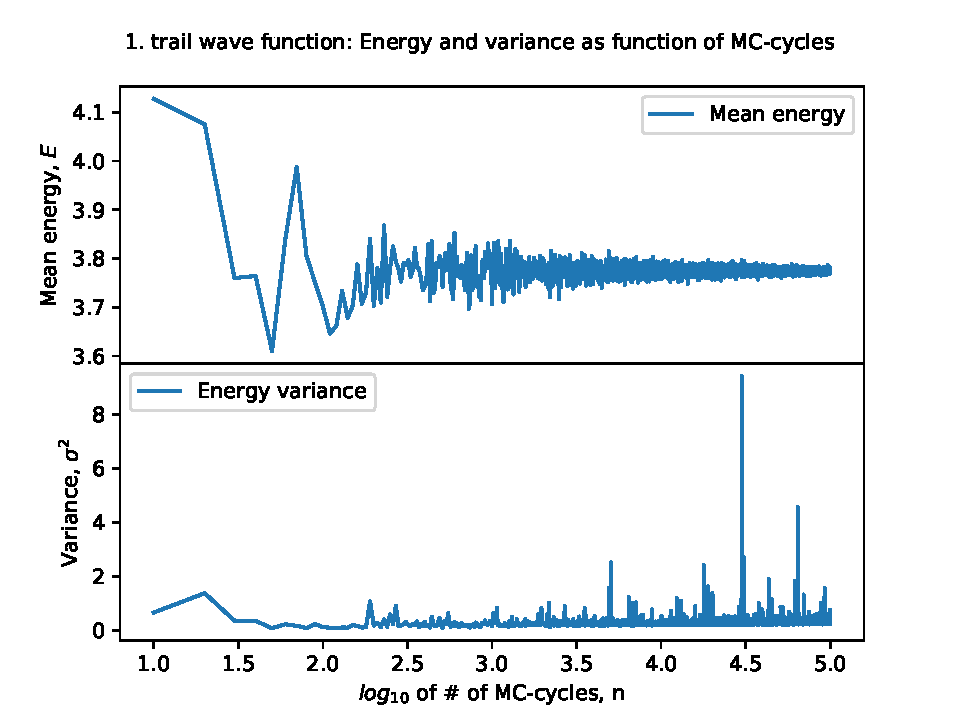
\includegraphics[scale=0.7]{../figures/plot_stability_trail_1.pdf}
    \caption{Plot of how the energy and variance of the 1st trail wave function evolves as the number of MC-cycles increases. Here; $\alpha=0.879096$.}
    \label{fig:stability_1}
\end{figure}
\begin{figure}[H]
    \centering
    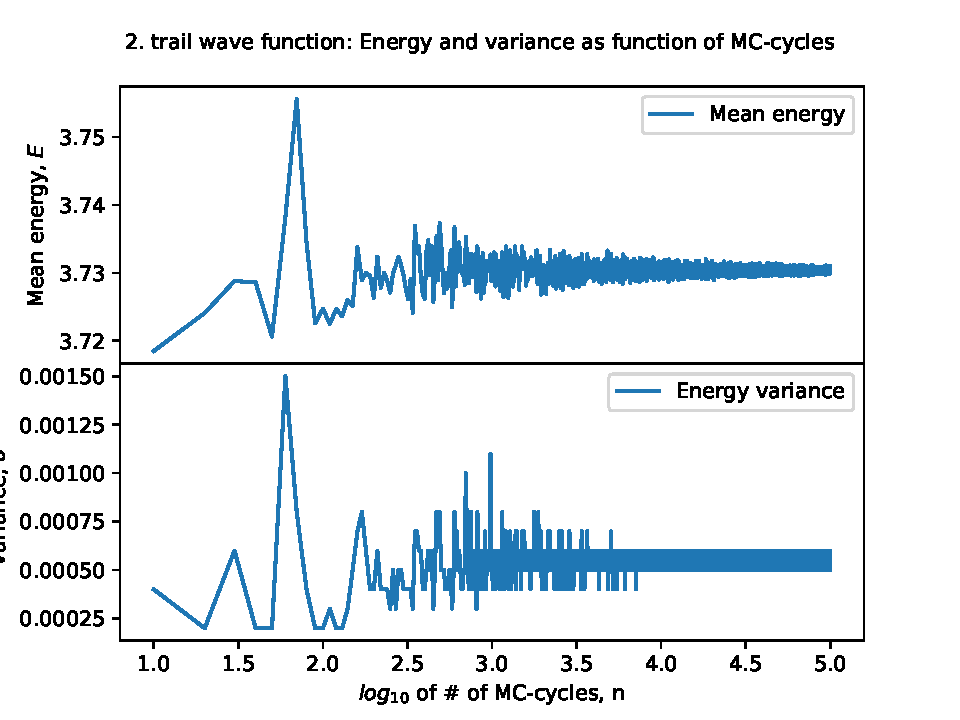
\includegraphics[scale=0.7]{../figures/plot_stability_trail_2.pdf}
    \caption{Plot of how the energy and variance of the 2nd trail wave function evolves as the number of MC-cycles increases. Here; $\alpha=0.994514$ and $\beta=0.28375$.}
    \label{fig:stability_2}
\end{figure}

\subsection{Optimal parameters and expectation values} \label{section:results:optimal}

The numerically calculated optimal parameters $\alpha$ and $\beta$ are given in Table \ref{tab:optimal}. With the use of these optimal values, the mean energies, variance and mean electron-electron distance is given in Table \ref{tab:expectation_values}. All values presented hereon is done with $10^6$ MC-cycles.

\begin{table}[htb]
    \centering
    \csvreader[tabular=lll,
        head=false,
        table head=\toprule,
        late after line=\\,
        late after first line=\\\midrule,
        table foot=\bottomrule,
        ]{../data/optimal_parameters.csv}{}{\csvcoli & \csvcolii & \csvcoliii}
        \caption{Optimal variational parameters.}
        \label{tab:optimal}
\end{table}

\begin{table}[htb]
    \centering
    \csvreader[tabular=lllllll,
        head=false,
        table head=\toprule,
        late after line=\\,
        late after first line=\\\midrule,
        table foot=\bottomrule,
        ]{../data/comparing_values.csv}{}{\csvcoli & \csvcolii & \csvcoliii & \csvcoliv}
        \caption{Comparison of the energies calculated using the VMC method and the Jacobi method from \textit{Project 2} to the exact value given in \cite{proj5}.}
        \label{tab:comparing}
\end{table}

\subsection{The Virial Theorem} \label{section:results:virial}

Figure \ref{fig:virial_trail_1} and \ref{fig:virial_trail_2} below presents the validity of the Virial Theorem for both trail wave functions with and without the electron-electron interactions.

\begin{figure}[H]
    \centering
    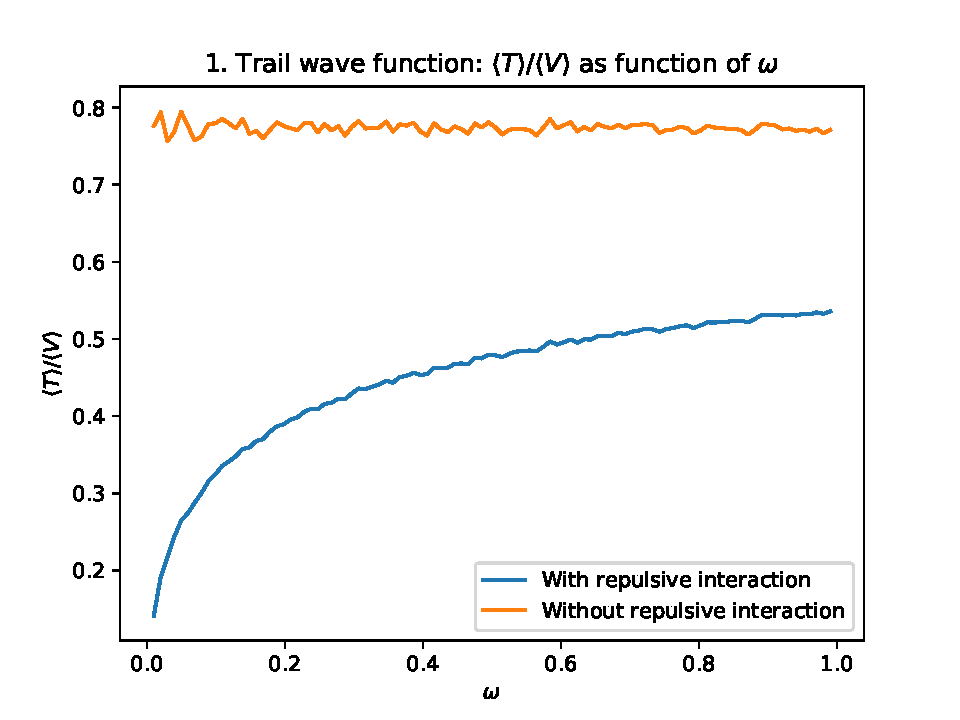
\includegraphics[scale=0.7]{../figures/plot_virial_trail_1.pdf}
    \caption{Plot of the ratio $\langle T\rangle / \langle V\rangle$ as function of HO frequency $\omega$ for $\Psi_{T1}$ with and without the repulsive electron-electron interactions. The optimal parameter for $\alpha$ is used.}
    \label{fig:virial_trail_1}
\end{figure}
\begin{figure}[H]
    \centering
    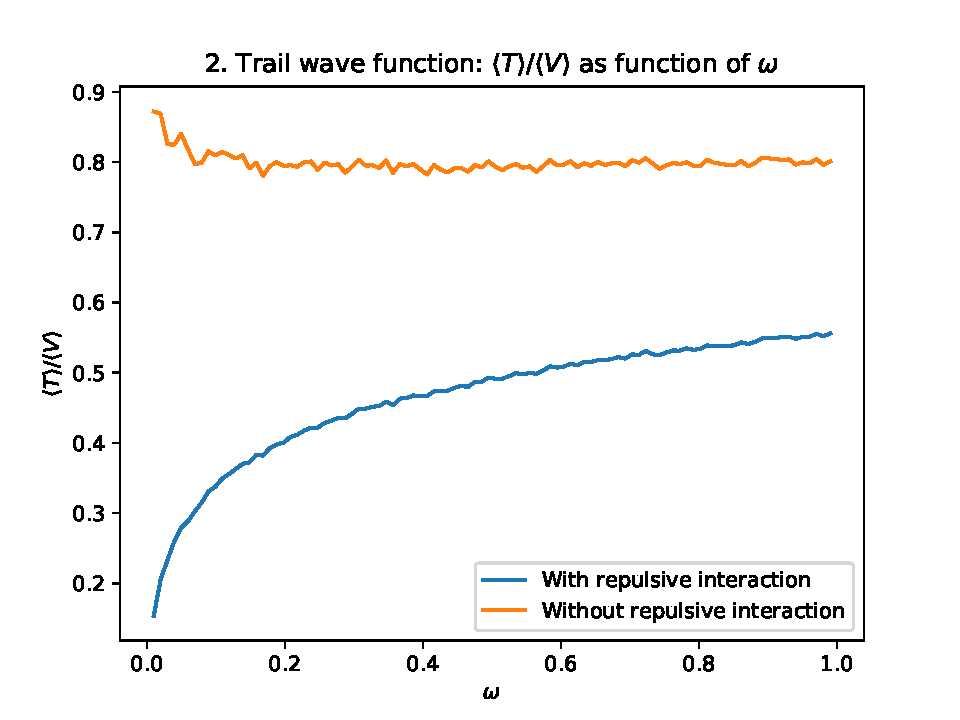
\includegraphics[scale=0.7]{../figures/plot_virial_trail_2.pdf}
    \caption{Plot of the ratio $\langle T\rangle / \langle V\rangle$ as function of HO frequency $\omega$ for $\Psi_{T2}$ with and without the repulsive electron-electron interactions. The optimal parameter for $\alpha$ and $\beta$ are used.}
    \label{fig:virial_trail_2}
\end{figure}

\section{Discussion} \label{section:discussion}
\subsection{Stability} \label{section:discussion:stability}
As seen in Figures \ref{fig:stability_1} and \ref{fig:stability_2} there is a clear increase in stability as the number of MC-cycles increases. The energy is clearly not stabilizing before at least $10^3$ MC-cycles is tried for both wave functions. After this, the spread in energy becomes smaller and an increase in number of cycles results in a more precise energy (in terms of decimals) for the respective wave functions. But, 

The the variance plots gives the same impression as that of the energies - there is a stabilization happening around $10^3$. These plots also gives a good indication of what the variance converges to, and whether or not the wave function (or chosen variational parameter) is good. The variance in Figure \ref{fig:stability_1} does have a different trend than that in Figure \ref{fig:stability_2}, because it shows some large peaks at high number of MC-cycles. These spikes in variance is probably caused by the fact that the 1st trail wave function is not a very good trail wave function. This will be discussed later in this section.

\subsection{Optimal parameters and expectation values} \label{section:discussion:optimal}
Section \ref{section:results:optimal} contains the most interesting data derived numerically in this report. First of is the optimal variational parameters presented in Table \ref{tab:optimal}. As shown in the lecture notes in FYS3150 \cite{Lec15}, the most correct wave function is obtained by minimizing either the energy or the variance. In this project, the variance was chosen to be minimized. The minimization algorithm was a sort of brute force minimization; where (for the second trail wave function) the first parameter, $\alpha$, was fixed, while the second, $\beta$, was minimized, then $\beta$ was fixed while $\alpha$ was minimized, and so fourth. This gave good result after a while, but consumed a bit much time (approximately 30 minutes). As seen in Table \ref{tab:expectation_values}, the variance was minimized down to the 4th decimal when using the 2nd wave function.

Table \ref{tab:proj2} from \textit{Project 2} presents some of the values calculated with the use of Jacobi's rotation algorithm and the analytical values by M. Taut. Comparing the best result from the VMC method to these is done in Table \ref{tab:comparing}. From this table, it is evident that that the most correct method is the VMC method with the second trail wave function which has a relative error of just $0.04898$. Though, the VMC method isn't the best in every aspect.

The expectation value of the energy from \textit{Project 2} is very close to the one derived with the second trail wave functions. But the expectation value of the first trail wave function has a relative error of $0.06141$ and is then the worst result. This coincides well with the high variance observed ($\sim 0.27$). Which in turn means that the first wave function is a bad trail wave function and gives a higher upper bound on the ground state of the quantum dots system than the second wave function.

Intuitively; we expect the electrons to be pushed close together as the harmonic oscillator potential increases. This would then ultimately give a high repulsive interaction between the electrons. The sixth and seventh column in Table \ref{tab:expectation_values} supports this expectation and presents an increasing electron-electron distance with decreasing $\omega$. This is also what was observed in \textit{Project 2} when the spatial probability density of the wave function was plotted for different $\omega_r$'s. This is shown in Figure \ref{fig:proj2_wave_functions}, where it's easy to see that high potential gives high probability of finding the electrons close together.

\subsection{The Virial Theorem} \label{section:discussion:virial}
The Virial Theorem tells us that we may predict that a HO-like system is to follow the linear dependance $\langle T\rangle = \langle V\rangle$. Figure \ref{fig:virial_trail_1} shows how the ratio $\langle T\rangle /\langle V\rangle$ depends on the HO frequency and the electron-electron interactions. Excluding the repulsive interactions of the electrons (orange graph); there is clearly a linear trend in the system. This is not shocking when looking at how the kinetic and potential energy is defined in the expression for $E_{L1}$ without the repulsive term (Equation \eqref{eq:local_energy_t1}). Assuming that the $3\alpha\omega$ term is small gives
\begin{align*}
    \langle T\rangle /\langle V\rangle \approx \frac{\frac{1}{2}\alpha^2\omega^2\left(r_1^2+r_2^2\right)}{\frac{1}{2}\omega^2\left(r_1^2+r_2^2\right)} \propto \alpha^2
\end{align*}
Where $\alpha^2=0.879096^2\approx 0.77$ is approximately the value on the y-axis in Figure \ref{fig:virial_trail_1} where the orange graph lies. In other words; this system satisfies the Virial Theorem.

Adding the repulsive interaction (blue graph), results in a very different case. Now, the ratio goes to $0$ as $\omega \rightarrow 0$. Looking at Table \ref{tab:expectation_values} in Appendix tells us that the mean distance between the electrons increases as $\omega$ decreases. So, a decrease in $\omega$ would result in a decrease in $1/r_{12}$ and since $\langle V\rangle$ is now a sum of $1/r_{12}$ and the HO potential energy; we would expect the graph to decrease with decreasing $\omega$. The reason why the graph goes to zero is that the nominator goes like $\omega^2$ and therefore goes faster to zero than $1/r_{12}$. This results in a small number divided by a (relatively) larger number, which gives zero. For large $\omega$, the repulsive term increases, but more slowly than the nominator and may perhaps eventually be neglected. This is seen as the graph slowly turns more and more linear. If these observations are correct; the graph should converge towards the one without repulsive interactions. This in terms gives reason to believe that for large $\omega$; the Virial Theorem is satisfied, but for small values of $\omega$, it is not.

Figure \ref{fig:virial_trail_2} demonstrates the Virial Theorem for the 2nd trail wave function with the Jastrow factor. This plot leads to exactly the same reasoning as the previous figure, but now there is an anomaly in the plot without repulsion. The anomaly is an increase in the ratio $\langle T\rangle /\langle V\rangle$ for small $\omega$. This can only be due to the second $\beta$-dependent term introduced in Equation \eqref{eq:local_energy_coulomb_t2} (which comes from the Jastrow factor). The first term, $\alpha\omega r_{12}$ is for small $\omega$ the dominating term, and this gives a positive contribution. While as $\omega$ grows larger, the other (negative) terms will dominate (as $1/r_{12}$ grows large too), and the graph becomes approximately constant. So, the second trail wave function satisfies the Virial Theorem in the same way as the first wave function, but the electron correlations from the Jastrow factor makes the Virial Theorem invalid for low frequencies in the non-repulsive system. 

\section{Conclusion} \label{section:conclusion}
Lets go!

As an after thought; maybe the Davidon-Fletcher-Powell (DFP) minimization algorithm (or similar ones) could have been better to use when minimizing the variance/energy. This the real bottle neck of the VMC when it came to time usage.

\section{Appendix} \label{section:appendix}
\subsection{Reproduce results} \label{section:appendix:reproduce}
To reproduce the data in this report; either compile the \texttt{cpp} files on GitHub or run the pre-compiled executable file called \texttt{exe} in the folder named \textit{cpp}. Running the executable gives 12 options:

\begin{itemize}
    \renewcommand\labelitemi{--}
    \item 0: Run all calculations (1-11).
    \item 1: Make plotfiles to plot minima of 1st wave function.
    \item 2: Make plotfiles to plot minima of 2nd wave function.
    \item 3: Minimize $\alpha$ of 1st wavefunction.
    \item 4: Minimize $\alpha$ and $\beta$ of 2nd wave function.
    \item 5: Make plotfiles to plot stability of 1st wave function.
    \item 6: Make plotfiles to plot stability of 2nd wave function.
    \item 7: Calculate optimal values of 1st wave function.
    \item 8: Calculate optimal values of 2nd wave function.
    \item 9: Make plotfiles to plot Virial Theorem of 1st wave function.
    \item 10: Make plotfiles to plot Virial Theorem of 2nd wave function.
    \item 11: Calculate values of the known wave function $\alpha\rho e^{-\alpha\rho}$.
\end{itemize}

Thereafter; run \texttt{plot\_data.py} to plot all data and save to pdf's.

\subsection{Tables and data} \label{section:appendix:tables}

Table \ref{tab:proj2} contains the experimental and exact values calculated in \textit{Project 2} while Table \ref{tab:expectation_values} contains the experimental expectation values of the mean energy, the electron-electron distance and the variance of each wave function. 

\begin{table}[htb]
    \centering
    \csvreader[tabular=llll,
        head=false,
        table head=\toprule,
        late after line=\\,
        late after first line=\\\midrule,
        table foot=\bottomrule,
        ]{../data/proj2.csv}{}{\csvcoli & \csvcolii & \csvcoliii & \csvcoliv}
        \caption{Experimental eigenvalues of the 2-electron system calculated in \textit{Project 2} and the analytic eigenvalues calculated using Eq. (16a) in \cite{Taut}. All as function of $\omega_r$. Here; $\omega_r=0.5$ implies $\omega=1$.}
        \label{tab:proj2}
\end{table}

\begin{table}[htb]
    \centering
    \csvreader[tabular=lllllll,
        head=false,
        table head=\toprule,
        late after line=\\,
        late after first line=\\\midrule,
        table foot=\bottomrule,
        ]{../data/expectation_values.csv}{}{\csvcoli & \csvcolii & \csvcoliii & \csvcoliv & \csvcolv & \csvcolvi & \csvcolvii}
        \caption{Expectation values of mean energy, electron-electron distance and the variance of the two trail wave functions as function of $\omega$. All calculations are done using the optimal values for $\alpha$ and $\beta$.}
        \label{tab:expectation_values}
\end{table}

Figure \ref{fig:minima_1} and Figure \ref{fig:minima_2} shows the energy of the trail wave functions as function of the variational parameters. Figure \ref{fig:proj2_wave_functions} is fetched from \textit{Project 2} and shows how the two-electron probability distribution is given in terms of $\omega_r$ and the position $\rho$.

\begin{figure}[H]
    \centering
    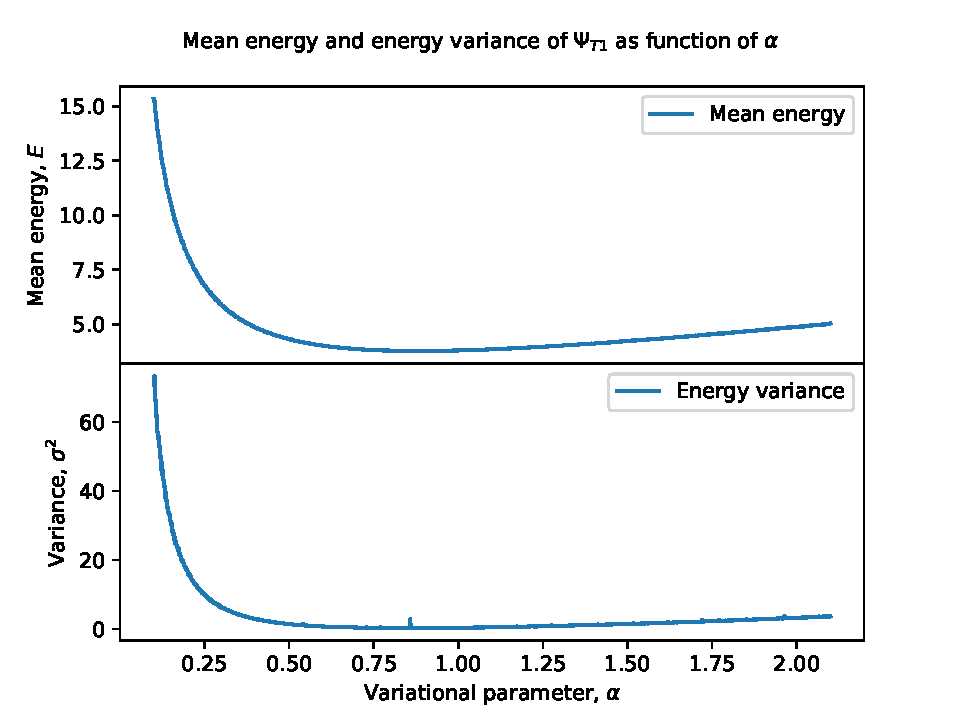
\includegraphics[scale=0.7]{../figures/plot_minima_trail_1.pdf}
    \caption{Plot of the mean energy and variance of the 1st trail wave function as function of $\alpha$.}
    \label{fig:minima_1}
\end{figure}
\begin{figure}[H]
    \centering
    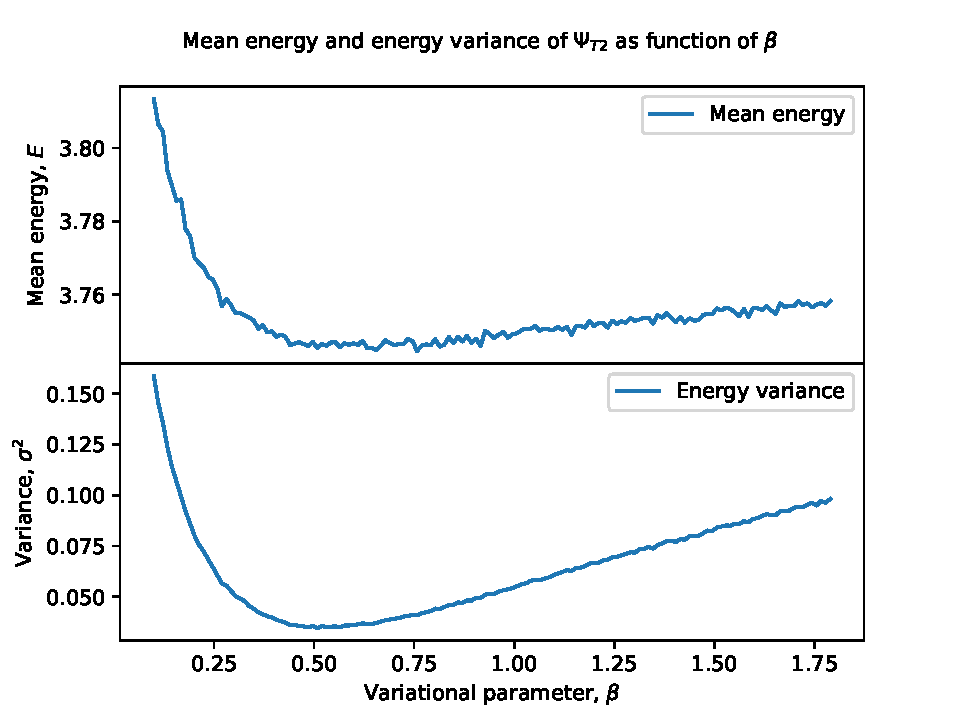
\includegraphics[scale=0.7]{../figures/plot_minima_trail_2.pdf}
    \caption{Plot of the mean energy and variance of the 2nd trail wave function as function of $\beta$. Here; $\alpha=0.879096$.}
    \label{fig:minima_2}
\end{figure}
\begin{figure}[H]
    \centering
    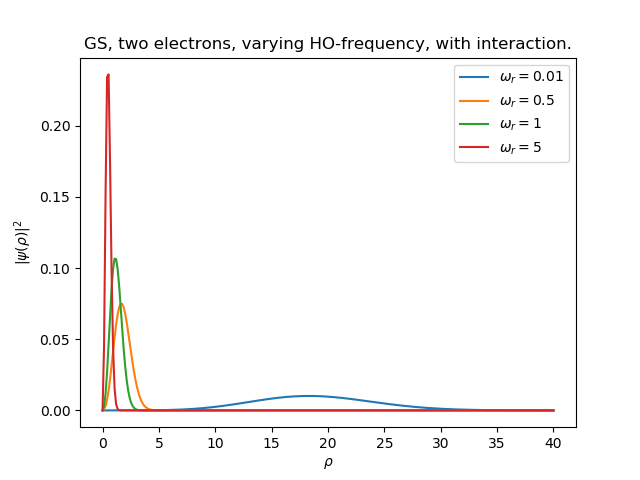
\includegraphics[scale=0.7]{../figures/project2_E_GS_with_interaction.png}
    \caption{Spatial probability distribution of different two-electron wave functions as function of the relative HO frequency, $\omega_r$, from \textit{Project 2}.}
    \label{fig:proj2_wave_functions}
\end{figure}

\subsection{Calculations} \label{section:appendix:calculations}
\subsubsection{Cusp conditions} \label{section:appendix:calculations:cusp}
As we already know that the cusp conditions are satisfied for the single electron (hydrogen) wave function, we do not need to evaluate the first trail wave function in Equation \eqref{eq:trail_one}, as it is a combination of this one. The second trail wave function in Equation \eqref{eq:trail_two} has a $r_{12}$ term, and we therefore need to evaluate if the condition
\begin{align*}
    \left[\frac{d\Psi_{Ti}}{dr_{12}}\right]_{r_{12}\rightarrow 0}=\frac{1}{2}\Psi(\frac{1}{2}(r_1+r_2),\frac{1}{2}(r_1+r_2),0)
\end{align*}
holds.

Calculating
\begin{align*}
    \left[\frac{d\Psi_{T2}}{dr_{12}}\right]=\left(\frac{2\left(1+\beta r_{12}\right)-r_{12}2\beta}{4\left(1+\beta r_{12}\right)^2}\right)\Psi_{T2}
\end{align*}
and as $r_{12}\rightarrow 0$ we have
\begin{align*}
    \left[\frac{d\Psi_{T2}}{dr_{12}}\right]_{r_{12}\rightarrow 0}=\frac{1}{2}e^0=\frac{1}{2}\Psi_{T2}(\frac{1}{2}(r_1+r_2),\frac{1}{2}(r_1+r_2),0)
\end{align*}
Which in terms means that the cusp condition is satisfied for both trail wave functions.

\subsubsection{Local energy of 2nd trail wave function} \label{section:appendix:calculations:energies}
First off, we simplify the expression for the second trail wave function as (excluding the normalization constant $C$)
\begin{align*}
    \Psi_{T2}=Ce^{-\frac{1}{2}\alpha\omega(r_1^2+r_2^2)}e^{\frac{r_{12}}{2(1+\beta r_{12})}}=A\cdot B
\end{align*}
where $A$ and $B$ are the respective exponential expressions and $B=e^{\frac{|r_1-r_2|}{2(1+\beta |r_1-r_2|)}}$. Acting with the squared del operator on $A\cdot B$ gives then
\begin{equation}
    \nabla_i^2\Psi_{T2}=\left(B\nabla_i^2A+2\nabla_iA\nabla_iB+A\nabla_i^2B\right)
    \label{eq:double_deriv}
\end{equation}
We calculate how the del operator acts on $A$
\begin{align*}
    \nabla_iA = -\alpha\omega \left(x_i+y_i+z_i\right)A
\end{align*}
\begin{align*}
    \nabla_i^2A = \left(\frac{d^2}{dx_i^2}+\frac{d^2}{dy_i^2}+\frac{d^2}{dz_i^2}\right)A
\end{align*}
\begin{align*}
    = \left[-\alpha\omega+\alpha^2\omega^2x_i^2-\alpha\omega+\alpha^2\omega^2y_i^2-\alpha\omega+\alpha^2\omega^2z_i^2\right]A
\end{align*}
\begin{align*}
    = \left[\alpha^2\omega^2\left(x_i^2+y_i^2+z_i^2\right)-3\alpha\omega\right]A
\end{align*}
\begin{align*}
    \rightarrow \nabla_i^2A = \left[\alpha^2\omega^2r_i^2-3\alpha\omega\right]A
\end{align*}
Using that $\frac{dr_{12}}{dx_i}=\frac{\left(x_i-x_{j\ne i}\right)}{r_{12}}$ we can find the expressions for how the del operator acts on $B$. We do this for just the $d/dx_i$-part first.
\begin{align*}
    \frac{d}{dx_i}B = \frac{\left(x_i-x_{j\ne i}\right)}{r_{12}\cdot 2\left(1+\beta r_{12}\right)^2}B
\end{align*}
\begin{align*}
    \frac{d^2}{dx_i^2} B = \left[\frac{r_{12}2\left(1+\beta r_{12}\right)^2}{r_{12}^2 4\left(1+\beta r_{12}\right)^4}-\frac{\left(x_i-x_{j\ne 1}\right)\left(\frac{\left(x_i-x_{j\ne 1}\right)}{r_{12}}2\left(1+\beta r_{12}\right)^2+r_{12}4\left(1+\beta r_{12}\right)\frac{\beta\left(x_i-x_{j\ne 1}\right)}{r_{12}}\right)}{r_{12}^2 4\left(1+\beta r_{12}\right)^4}\right]B\\
    +\left[\left(\frac{\left(x_i-x_{j\ne i}\right)}{r_{12}\cdot 2\left(1+\beta r_{12}\right)^2}\right)^2\right]B
\end{align*}
Defining
\begin{align*}
    F_i^{(x)}=\frac{\left(x_i-x_{j\ne i}\right)^2}{r_{12}^2}
\end{align*}
where $\left(F_i^{(x)}+F_i^{(y)}+F_i^{(z)}\right)=1$. We can write
\begin{align*}
    \frac{d^2}{dx_i^2} B = \left[\frac{1}{r_{12}2\left(1+\beta r_{12}\right)^2}- F_i^{(x)}\frac{1}{r_{12}2\left(1+\beta r_{12}\right)^2}-F_i^{(x)}\frac{2\beta}{2\left(1+\beta r_{12}\right)^3}+F_i^{(x)}\frac{1}{4\left(1+\beta r_{12}\right)^4}\right]B
\end{align*}
So that the del operators on $B$ gives
\begin{align*}
    \nabla_i B = \frac{\left(x_i-x_{j\ne i}\right)+\left(y_i-y_{j\ne i}\right)+\left(z_i-z_{j\ne i}\right)}{r_{12}\cdot 2\left(1+\beta r_{12}\right)^2}B
\end{align*}
and
\begin{align*}
    \nabla_i^2 B = \left[3\cdot\frac{1}{r_{12}2\left(1+\beta r_{12}\right)^2}-\left(1\right)\cdot\frac{1}{r_{12}2\left(1+\beta r_{12}\right)^2}-\left(1\right)\cdot\frac{2\beta}{2\left(1+\beta r_{12}\right)^3}+\left(1\right)\cdot\frac{1}{4\left(1+\beta r_{12}\right)^4}\right]B
\end{align*}
\begin{align*}
    = \frac{1}{2\left(1+\beta r_{12}\right)^2}\left[\frac{2}{r_{12}}-\frac{2\beta}{1+\beta r_{12}}+\frac{1}{2\left(1+\beta r_{12}\right)^2}\right]
\end{align*}
Precalculating the expression
\begin{align*}
    2\nabla A_1\nabla B_1+2\nabla A_2\nabla B_2
\end{align*}
\begin{align*}
    =-\frac{2\alpha\omega}{2\left(1+\beta r_{12}\right)^2}\left(\frac{x_1\left(x_1-x_2\right)+x_2\left(x_2-x_1\right)+y_1\left(y_1-y_2\right)+y_2\left(y_2-y_1\right)+z_1\left(z_1-z_2\right)+z_2\left(z_2-z_1\right)}{r_{12}}\right)
\end{align*}
\begin{align*}
    = -\frac{2\alpha\omega}{2\left(1+\beta r_{12}\right)^2}\left(\frac{x_1^2+y_1^2+z_1^2-2\left(x_1x_2+y_1y_2+z_1z_2\right)+x_2^2+y_2^2+z_2^2}{r_{12}}\right)
\end{align*}
\begin{align*}
    = -\frac{2\alpha\omega}{2\left(1+\beta r_{12}\right)^2}\left(\frac{\boldsymbol{r_1}\cdot\boldsymbol{r_1}-2\boldsymbol{r_1}\cdot\boldsymbol{r_2}+\boldsymbol{r_2}\cdot\boldsymbol{r_2}}{r_{12}}\right)
\end{align*}
\begin{align*}
    = -\frac{2\alpha\omega}{2\left(1+\beta r_{12}\right)^2}\left(\frac{|\boldsymbol{r_1}-\boldsymbol{r_2}|^2}{r_{12}}\right)
\end{align*}
\begin{align*}
    = -\frac{2\alpha\omega}{2\left(1+\beta r_{12}\right)^2}r_{12}
\end{align*}
Now, writing the squared del operator acting on the second trail wave function as
\begin{align*}
    \nabla_i^2 \Psi_{T2}=D_i\Psi_{T2}
\end{align*}
where
\begin{align*}
    D_i=\left[\alpha^2\omega^2 r_i^2-3\alpha\omega\right]+2\nabla_i A\nabla_i B+\frac{1}{2\left(1+\beta r_{12}\right)^2}\left[\frac{2}{r_{12}}+\frac{1}{2\left(1+\beta r_{12}\right)^2}-\frac{2\beta}{1+\beta r_{12}}\right]
\end{align*}
Using the total Hamiltonian from Equation \eqref{eq:hamiltonian_total}, we may now get the expression for the local energy of the second trail wave function with the use of Equation \eqref{eq:local_energy} as
\begin{align*}
    E_{L2}=-\frac{1}{2}D_1-\frac{1}{2}D_2+\frac{1}{2}\omega^2r_1^2+\frac{1}{2}\omega^2r_2^2+\left(\frac{1}{r_{12}}\right)
\end{align*} 
\begin{align*}
    =E_{L1}-\left(-\frac{1}{2}\right)\frac{2}{2\left(1+\beta r_{12}\right)^2}\alpha\omega r_{12}-\left(\frac{1}{2}\right)\cdot 2\frac{1}{2\left(1+\beta r_{12}\right)^2}\left[\frac{2}{r_{12}}+\frac{1}{2\left(1+\beta r_{12}\right)^2}-\frac{2\beta}{1+\beta r_{12}}\right]
\end{align*}
\begin{align*}
    =E_{L1}+\frac{1}{2\left(1+\beta r_{12}\right)^2}\left[\alpha\omega r_{12}-\frac{1}{2\left(1+\beta r_{12}\right)^2}-\frac{2}{r_{12}}+\frac{2\beta}{1+\beta r_{12}}\right]
\end{align*}
where $E_{L1}$ is as in Equation \eqref{eq:local_energy_coulomb_t1} derived in Section \ref{section:theory:energies}.  

\printbibliography

\end{document}
